\chapter{Evaluation}

Dieses Kapitel widmet sich einer umfassenden Analyse der Relevanz und Effektivität des GReQL Converters als innovatives
Werkzeug. Spezifisch zielt diese Abschnitt darauf ab, die grundlegende Frage zu beantworten, ob dieses Instrument
tatsächlich im akademischen und pädagogischen Kontext nützlich ist. Um dieses Ziel zu erreichen, ist es von größter
Wichtigkeit, eine systematische Herangehensweise zu verfolgen, die die Anwendung verschiedener Bewertungsmethoden
beinhaltet, um die Vorzüge und Effektivität des GReQL Converters nachzuweisen. Dieses Kapitel behandelt ausführlich die
angewandten Ansätze zur Prüfung des GReQL Converters, die Datensammlungsmethoden und die durchgeführten Analysen zur
Messung seiner Nützlichkeit. Letztendlich geht es darum, empirisch festzustellen, ob dieses Werkzeug konkrete Vorteile
und einen signifikanten Mehrwert für Lehrende und Lernende bietet.

\section{Erreichte Ziele}\label{sec:erreichte-ziele}

Die Untersuchung der Effizienz und Funktionalität des GReQL Converters als Instrument zur Extraktion relevanter
GReQL-Regeln aus einer UML-Diagrammannotation, die mittels PlantText zur Evaluation von UML-Diagrammen erstellt wurde,
stellt eine essenzielle Fragestellung dar, welche eine systematische und tiefgehende Herangehensweise erfordert. In dem
Implementierungskapitel (siehe Kapitel~\ref{ch:implementierung}) wurden diverse Regeln vorgestellt, begleitet von einer detaillierten Erläuterung des
spezifischen Extraktionsprozesses für jede dieser Regeldefinitionen. Gleichwohl erwies sich eine umfassende Testphase
als unverzichtbar, um eine eingehende Evaluierung der Leistungsfähigkeit jeder einzelnen Regel zu ermöglichen.

Zur Durchführung dieser Evaluierungen wurden verschiedene Testverfahren appliziert, welche eine Vielzahl von Szenarien
und Variationen abdeckten, mit dem Ziel, die Effizienz der durch den GReQL Converter generierten Regeldefinitionen
im Detail zu beurteilen. Der Testprozess kann in vier diskrete Schritte unterteilt werden:

\begin{enumerate}[itemsep=3pt, parsep=3pt]
    \item Initiale Generierung eines Diagramms mithilfe von PlantText, wobei dieses Diagramm gezielt konzipiert wurde,
um die spezifischen Merkmale der zu evaluierenden Regel zu inkorporieren. Zum Beispiel wurde ein Diagramm erstellt,
welches eine Aggregation zwischen zwei Klassen darstellte, um eine Regel zur Aggregation zu prüfen.
    \item Erstellung eines Evaluationsdiagramms (welches in diesem Kontext mittels BOUML modellisiert wurde), welches von
den generierten Regeldefinitionen bewertet werden sollte.
    \item Extraktion der verschiedenen Regeldefinitionen aus dem PlantText-Code.
    \item Evaluierung mithilfe der GReQL-Engine von JACK, um festzustellen, ob die Regeldefinitionen die Aggregation
im Diagramm effektiv erkannt haben.
\end{enumerate}

Parallelen dazu wurde besonderes Augenmerk auf die Identifikation von falsch positiven (False Positiv) Ergebnissen
gerichtet, welche den Eindruck einer korrekten Funktionsweise des Werkzeugs erwecken könnten, obwohl dem nicht so ist.
Hierzu wurde eine sorgfältige Analyse des generierten Codes durchgeführt, und die Protokolle der GReQL-Engine wurden
überprüft, um die präzise Identifikation der Aggregationsregel sicherzustellen. Es sei hervorgehoben, dass dieser
gewissenhafte Überprüfungsprozess in systematischer Weise auf alle vorab definierten Regeldefinitionen der
Implementierungsphase angewandt wurde.

Im Anschluss an die individuelle Prüfung jeder Regeldefinition erfolgte eine Evaluierung anhand zunehmend komplexerer
Diagramme. Das Ziel bestand darin, mehrere Funktionen simultan zu bewerten und zu ermitteln, ob die Existenz mehrerer
Verknüpfungen zwischen verschiedenen Elementen im Diagramm spezifische Regeldefinitionen nicht beeinträchtigte. Die
Bedingungen, die zu potenziellen Konflikten führen könnten, wurden somit eingehend untersucht, und der GReQL Converter
wurde bei jeder Fehlererkennung oder -identifikation angepasst, um seine Effizienz zu steigern.

In einem darauffolgenden Schritt wurden verschiedene gängige Übungen zu UML-Diagrammen selektiert, um die akademische
Leistung der Studierenden an der Universität zu evaluieren. Unter diesen Übungen findet sich das Diagramm ``Mendelssohn
\& Sohn Maschinenbau GmbH'', welches im Rahmen des Kurses ``Einführung in die Unified Modeling Language'' an der
Universität Potsdam zum Einsatz kam (siehe Abbildung~\ref{fig:bau_gmbh}). Dieses spezifische Diagramm weist signifikante
Ähnlichkeiten zu den traditionellen Modellen auf, die in universitären Prüfungskontexten verwendet werden, wodurch es
sich als exemplarisches Testobjekt zur Ermittlung der Leistungsfähigkeit des GReQL Converters erweist.

Zu diesem Ziel wurde das Musterdiagramm, das als Repräsentation der Übungsvorlage diente, mittels des Werkzeugs
BOUML modelliert. Anschließend erfolgte die Extraktion der XMI-Datei, welche als Bewertungsinstrument diente. Parallel
dazu wurde die Anwendung von PlantText zur Erstellung der Musterdiagrammvorlage in Erwägung gezogen, wobei der GReQL
Converter im Anschluss dazu verwendet wurde, um die Regeln gemäß dem vorab beschriebenen Verfahren formal zu erfassen.
Subsequent zur Extraktion der Regeldefinitionen und der willkürlichen Punktevergabe für jede einzelne Regel, unterzog
man diese Regeldefinitionen einer Evaluation im Rahmen des GReQL-Motors von JACK.

Hervorzuheben ist, dass für ein mittelkomplexes Diagramm wie das genannte insgesamt \textbf{82 GReQL-Regeln} generiert
wurden. Nach abschließenden Tests ergab sich, dass der GReQL-Motor eine Erfolgsrate von 100\% aufwies, was auf die
korrekte Funktionalität der erzeugten Regeldefinitionen hinweist. Dieser Erfolg illustriert eindrucksvoll die Befähigung
des GReQL Converters zur effektiven Evaluierung von UML-Diagrammen, insbesondere jener von erhöhter Komplexität.

\begin{figure}[h]
    \centering
    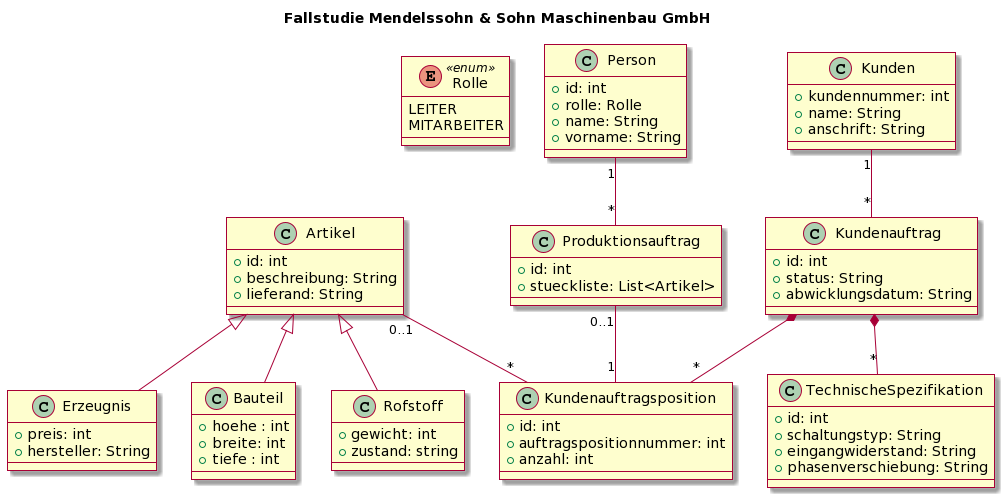
\includegraphics[width=16cm]{images/bau_gmbh_plantText}
    \caption{Fallstudie UML - Klassendiagramm}
    \label{fig:bau_gmbh}
\end{figure}

In Bezug auf die Leistungen, die dem GReQL Converter zugeschrieben werden können, lassen sich folgende Punkte
feststellen:

\begin{enumerate}[itemsep=3pt, parsep=5pt]
    \item Der GReQL Converter ermöglicht die umfassende Bewertung eines Diagramms. Im vorherigen Beispiel ermöglichte er
die Generierung von 82 Regeln, eine Aufgabe, die besonders mühsam und fehleranfällig wäre, wenn sie manuell von einem
Lehrer durchgeführt würde.
    \item Der GReQL Converter führt Bewertungen äußerst präzise durch und verhindert somit potenzielle Fehler, die
Lehrer bei manuellen Bewertungen begehen könnten.
    \item Der GReQL Converter verhindert Fehler in Bezug auf die Syntax und Formulierung von Regeln, insbesondere
solche, die bereits vom Tool definiert sind, was den Benutzer von Sorgen in Bezug auf diese Aspekte entlastet.
    \item Darüber hinaus ist eine direkte Interaktion mit dem GReQL-Code nicht mehr erforderlich, da der Benutzer die
Regeln problemlos ändern kann, indem er die generierten Objekte nach dem Schritt der syntaktischen Analyse verwendet,
was den Bearbeitungsprozess vereinfacht.
    \item Der GReQL Converter erleichtert erheblich das Verständnis des GReQL-Codes, indem er klaren, lesbaren und
zugänglichen Code generiert, was es Dritten ermöglicht, seine Funktionsweise zu verstehen und bei Bedarf Änderungen
vorzunehmen.
    \item Darüber hinaus berücksichtigt das Design des Tools die Vielfalt grundlegender Varianten in UML-Diagrammen,
was seine Vielseitigkeit und Anpassungsfähigkeit stärkt.
\end{enumerate}

Wenn man diese Vorteile mit den in Teil drei aufgeführten Problemen vergleicht, die die
Problemanalyse (siehe Kapitel~\ref{ch:problemanalyse}) behandelten, steht außer Frage, dass der GReQL Converter seine Rolle als
Hilfsmittel bei der Erstellung von GReQL-Code für die Bewertung von Klassendiagrammen erfüllt und Lehrern erheblich
Zeit spart. Im nächsten Abschnitt wird eine Studie durchgeführt, um zu ermitteln, ob Lehrende diese Ansicht teilen.

\section{Interview zur Bewertung des GReQL Converters}

Im vorherigen Kapitel wurde der GReQL Converter auf seine Funktionen hin getestet, um potenzielle Fehler zu erkennen und
zu beheben. Es war jedoch von entscheidender Bedeutung, externe Rückmeldungen und Kommentare einzuholen, um weitere
Verbesserungsansätze zu identifizieren, neue Ideen zu generieren und die Grenzen des Tools aufzuzeigen. Aus diesem Grund
wurde beschlossen, Interviews mit verschiedenen wissenschaftlichen Mitarbeitern durchzuführen, die bereits Erfahrung
mit GReQL-Code haben, um das Tool zu testen.

Das Interview erwies sich als das geeignetste Modell, da es bereits die Möglichkeit bietet, direkte Fragen zu stellen
und ein lebhafteres Feedback zu erhalten sowie detaillierte und umfassende Antworten vom Befragten zu erhalten. Darüber
hinaus ermöglicht das Interviewformat eine gewisse Flexibilität, da zukünftige Fragen je nach den erhaltenen Antworten
angepasst werden können. Dieses Format erleichtert auch die Kontextualisierung. Falls eine Frage nicht verstanden wird,
kann der Befragte Nachfragen stellen, um im Kontext zu bleiben. Im folgenden Abschnitt wird zunächst die
Interviewkonzeption sowie der Prozess und die Ergebnisse des Interviews diskutiert.

\subsection{Konzeption des Interviews}

Das Ziel des Interviews besteht darin, das Feedback verschiedener Lehrer zum GReQL Converter zu sammeln und die
Möglichkeiten zur Verbesserung des Tools zu erörtern. Am Ende des Interviews wird es möglich sein festzustellen, ob
das Tool einen echten Nutzen für die Benutzer hat und ob es sinnvoll ist, seine Entwicklung fortzusetzen. Um dies zu
erreichen, war es zunächst erforderlich, die verschiedenen Lehrer anhand bestimmter Kriterien zu qualifizieren,
darunter:

\begin{enumerate}[itemsep=3pt, parsep=5pt]
    \item Die Lehrer sollten bereits wissen, was GReQL ist.
    \item Die Lehrer sollten bereits GReQL-Code geschrieben haben, um ein UML Klassendiagramm zu bewerten.
\end{enumerate}

Das Interview erstreckt sich tatsächlich über fünf Phasen, von der Vorbereitung bis zum Fragebogen:

\subsubsection{PHASE 1: Vorbereitung auf das Interview}

Während des Interviews sollte der Schwerpunkt auf dem GReQL Converter liegen. Um zu verhindern, dass die Lehrer
während des Interviews mit dem Schreiben von PlantText-Code beschäftigt sind, wurde beschlossen, sicherzustellen,
dass die Lehrer vor dem Interview den PlantText-Code schreiben, den sie während des Interviews benötigen werden. Zu
diesem Zweck sollen die interviewten Personen eine Übung durchführen, die sie mit dem PlantText-Tool und plantUML
vertraut macht.

Bei der Einladung zum Interview wurde ein Bild ausgewählt und an die Lehrer gesendet, das bereits sein äquivalentes XMI
generiert hat, das später verwendet wird, um den generierten GReQL-Code auf JACK zu testen. Da das Hauptziel darin
besteht, GReQL-Code aus PlantText zu generieren, sollen die Lehrer versuchen, die Musterlösung auf PlantText zu
reproduzieren:

\begin{enumerate}[itemsep=5pt, parsep=5pt]
    \item Wenn sie dies schaffen, müssen sie ihren PlantText-Code lediglich mit dem GReQL Converter annotieren, die
Lösung auf JACK testen und die während des Interviews gestellten Fragen beantworten.
    \item Wenn sie dies nicht geschafft haben, wird ihnen der PlantText-Code zur Verfügung gestellt und erklärt, wie
dieser Code erstellt wurde, einschließlich einiger Feinheiten. Anschließend sollen sie diesen PlantText-Code mit dem
GReQL Converter annotieren und die während des Interviews gestellten Fragen beantworten.
\end{enumerate}

Es ist auch wichtig, den Lehrern die Dokumentation zum GReQL Converter sowie den Zugang zum Tool zur Verfügung zu
stellen, damit sie es vor dem Interview testen und sich damit vertraut machen können, wenn ihre Verfügbarkeit dies
zulässt.

\subsubsection{PHASE 2: Einführung in das Interview}

In dieser Phase geht es darum, den GReQL Converter vorzustellen, seine Feinheiten, Funktionen sowie seine Verwendung und
Dokumentation zu präsentieren. Das Ziel dieser Phase besteht darin, die Lehrer mit dem Tool vertraut zu machen und
ihnen alle notwendigen Informationen für den weiteren Verlauf zur Verfügung zu stellen.

\subsubsection{PHASE 3: Annotation des PlantText-Codes}

In dieser Phase müssen sich die Lehrer auf die Annotation des PlantText-Codes im GReQL Converter konzentrieren. Sie
verwenden das Tool zur Generierung von GReQL-Code.

\subsubsection{PHASE 4: Test des generierten GReQL-Codes}

In dieser Phase müssen die Lehrer den generierten GReQL-Code auf JACK testen. Zu diesem Zweck wurden entsprechende
Übungen bereits auf der Plattform vorbereitet, um den Prozess zu erleichtern. Sie müssen lediglich ihren GReQL-Code
sowie das zuvor vorbereitete XMI eingeben, um ihn zu testen.

\subsubsection{PHASE 5: Fragebogen}

Am Ende des Interviews werden den Lehrern eine Reihe von vorbereiteten Fragen gestellt, um ihre Erfahrungen, Meinungen
und Verbesserungsvorschläge für den GReQL Converter zu bewerten. Die während des Interviews gestellten Fragen sind
wie folgt:

\begin{enumerate}[itemsep=5pt, parsep=5pt]
    \item \textbf{Einführung in das Tool:}
    \begin{enumerate}
        \item Können Sie kurz erklären, was das Tool GReQL Converter Ihrer Meinung nach ist?
        \item Haben Sie bereits ähnliche Tools zur Generierung von GReQL-Code aus UML-Diagrammen verwendet?
    \end{enumerate}
    \item \textbf{Benutzererfahrung:}
    \begin{enumerate}
        \item Wie empfanden Sie die Benutzeroberfläche des GReQL Converters in Bezug auf Benutzerfreundlichkeit?
        \item Können Sie die Schritte beschreiben, die Sie unternommen haben, um das Tool zu verwenden, von der
        Code-Importierung aus PlantText bis zur Generierung von GReQL-Code?
        \item Ist das Tool intuitiv?
        \item Konnten Sie auf einen Blick verstehen, was Sie tun mussten?
        \item Gab es Probleme oder Hindernisse bei der Verwendung des Tools?
    \end{enumerate}
    \item \textbf{Dokumentation:}
    \begin{enumerate}
        \item Haben Sie die Dokumentation des GReQL Converters konsultiert?
        \item Wenn ja, wie fanden Sie sie in Bezug auf Klarheit und Nützlichkeit?
        \item Gibt es Aspekte des Tools oder seiner Funktionsweise, die Sie in der Dokumentation nicht
        verstanden haben und die Sie gerne darin gefunden hätten?
    \end{enumerate}
    \item \textbf{Generierung von GReQL-Regeln:}
    \begin{enumerate}
        \item Wie würden Sie die Genauigkeit des Tools bei der Generierung von GReQL-Regeln aus mit PlantText
        erstellten UML-Diagrammen bewerten?
        \item Gab es Fehler oder Inkonsistenzen in den generierten Regeln?
    \end{enumerate}
    \item \textbf{Vergleich des Tools mit der manuellen Methode:}
    \begin{enumerate}
        \item Wie würden Sie die Effizienz des GReQL Converters im Vergleich zur manuellen Erstellung von GReQL-Regeln
        aus UML-Diagrammen in Bezug auf Zeitersparnis und Genauigkeit bewerten?
        \item Können Sie konkrete Beispiele nennen, in denen das Tool besonders nützlich oder weniger effektiv als
        die manuelle Methode war?
    \end{enumerate}
    \item \textbf{Verbesserungsvorschläge:}
    \begin{enumerate}
        \item Haben Sie Vorschläge zur Verbesserung der Benutzeroberfläche oder der Funktionen des GReQL Converters?
        \item Gibt es zusätzliche Funktionen, die Sie gerne im Tool sehen würden?
    \end{enumerate}
    \item \textbf{Nützlichkeit und Relevanz:}
    \begin{enumerate}
        \item Halten Sie das Tool GReQL Converter im Kontext der Bewertung von UML-Diagrammen für nützlich?
        \item Warum oder warum nicht?
    \end{enumerate}
    \item \textbf{Gesamtbewertung:}
    \begin{enumerate}
        \item Auf einer Skala von 1 bis 5, wobei 1 ``nutzlos'' und 5 ``äußerst nützlich'' bedeutet, wie würden Sie die
        Nützlichkeit des GReQL Converters bewerten?
        \item Auf einer Skala von 1 bis 5, wobei 1 ``sehr schlecht'' und 5 ``ausgezeichnet'' bedeutet, wie würden Sie
        das Design des GReQL Converters bewerten?
        \item Auf einer Skala von 1 bis 5, wobei 1 ``sehr schlecht'' und 5 ``ausgezeichnet'' bedeutet, wie würden Sie
        die Benutzerfreundlichkeit des GReQL Converters bewerten?
        \item Würden Sie dieses Tool anderen Fachleuten empfehlen, die mit UML-Diagrammen zur Bewertung arbeiten?
    \end{enumerate}
    \item \textbf{Allgemeines Feedback:}
    \begin{enumerate}
        \item Haben Sie weitere Kommentare, Vorschläge oder Beobachtungen, die Sie zum GReQL Converter teilen möchten?
    \end{enumerate}
\end{enumerate}

Die grundlegende Struktur der Interviews und die Wahl der Fragen wurden maßgeblich von den Erkenntnissen und Ratschlägen
des Autors Ian Brace in seinem Werk ``Questionnaire Design: How to Plan, Structure and Write Survey Material for
Effective Market Research'' beeinflusst~\cite{brace2018questionnaire}. Dieses Buch bietet umfassende Einblicke in
bewährte Methoden zur Gestaltung von Fragen und zur Strukturierung von Umfragen, die sich auch auf die
Interviewkonzeption übertragen lassen. Bei der Gestaltung der Fragen zur Benutzererfahrung und Benutzerfreundlichkeit
wurde das Buch ``Designing and Conducting Survey Research: A Comprehensive Guide'' von Louis M. Rea und Richard
A. Parker~\cite{rea2014designing} herangezogen, um die Best Practices für die Benutzerfreundlichkeit von Fragen zu
verstehen. Online-Umfrageplattformen wie SurveyMonkey~\cite{monkey} dienten als Inspiration für die Erstellung des
Interviewleitfadens und halfen bei der Identifizierung bewährter Praktiken zur Erstellung von Fragen und zur
Strukturierung von Umfragen. Im kommenden Abschnitt steht die Präsentation einer Auswahl der Ergebnisse nach den
Interviews im Vordergrund.


\subsection{Ergebnisse des Interviewverfahrens}

Die Interviews wurden mit einer Gruppe von fünf wissenschaftlichen Mitarbeitern von zwei Hochschulen geführt, nämlich
der Universität Duisburg-Essen und der Technischen Hochschule Köln (siehe Tabelle~\ref{tab:personnen}).

\begin{table}
    \centering
    \caption{Befragte wissenschaftliche Mitarbeiter} \label{tab:personnen}
    \begin{adjustbox}{scale=0.9}
        \begin{tabular}{ll}
            \toprule
            \textbf{Hochschule} & \textbf{Lehrkraft} \\
            \midrule
            Universität Duisburg Essen & Dr. Michael Striewe \\
            \midrule
            Universität Duisburg Essen & Tobias Stottrop \\
            \midrule
            Universität Duisburg Essen & Christoph Olbricht \\
            \midrule
            Technische Hochschule Köln & Paul Hufnagel \\
            \midrule
            Technische Hochschule Köln & Prof. Dr. Mario Winter \\
            \bottomrule
        \end{tabular}
    \end{adjustbox}
\end{table}

\subsubsection{Interview mit Christoph Olbricht}
Christoph Olbricht, wissenschaftlicher Mitarbeiter an der Universität Duisburg-Essen, hat bereits GReQL-Code für die
Auswertung von Java-Übungen geschrieben. Allerdings fehlt ihm Erfahrung in der Auswertung von UML-Diagrammen. Das
Interview begann mit einer Vorstellung des GReQL Converters, einschließlich seiner Funktionen und Dokumentation. Vor
dem Interview erhielt Herr Olbricht per E-Mail ein UML-Diagramm, für das er im Voraus PlantText-Code schrieb. Während
des Interviews übertrug er den Code auf den GReQL Converter, annotierte ihn und führte mehrere Modifikationen durch.
Nachfolgend generierte er GReQL-Code, der erfolgreich auf JACK getestet wurde, wobei eine Bewertung von 100\% erreicht
wurde. Am Ende des Interviews wurden Fragen aus dem vorherigen Abschnittsfragebogen gestellt, um ein spezifisches
Feedback zum Tool zu erhalten.

\begin{enumerate}[itemsep=8pt, parsep=5pt]
    \item \textbf{Einführung in das Tool:}

    Gemäß seinen exakten Worten zum GReQL Converter: ``Mit diesem Tool können wir auf einfache und intuitive Weise
    GReQL-Code aus PlantText generieren und ihn auf sehr angenehme Art und Weise anpassen.'' Er hatte zuvor kein
    ähnliches Tool für die Generierung von GReQL-Code für Klassendiagramme verwendet.

    \item \textbf{Benutzererfahrung:}

    Entsprechend seiner exakten Worte zur Benutzerfreundlichkeit der Anwendung: ``Unheimlich angenehm. Vorher hatten wir
    ein ähnliches Tool für Java, aber dabei musste man seinen Java-Code einlesen und dann einen GReQL-Code einwerfen,
    um zu sehen, ob es funktioniert. Es war nur zum Testen gedacht. Bei deinem Tool ist es jedoch besonders angenehm,
    dass man die komplette Regel direkt erhält und sie nach Bedarf anpassen kann. Dadurch muss ich GReQL eigentlich
    nicht beherrschen, was für unsere Kunden unheimlich nützlich wäre.''

    Herr Olbricht fand das Tool intuitiv und war überrascht, dass die Regeln direkt generiert wurden, ohne dass eine
    umfangreiche Vorarbeit mit Annotationen geleistet werden musste. Das Tool macht viel mehr, als er erwartet hatte.
    Er hätte gerne einen Text gehabt, der den Prozess der Regelgenerierung sowie die Grundregeln klar erklaert und er
    betont am Ende: ``Aber intuitiv genug war das definitiv''.

    \item \textbf{Dokumentation:}

    Er lobte die Dokumentation als ausgezeichnet, ausgewogen und präzise. Die Menge an Inhalten wurde als angemessen empfunden.
    
    \item \textbf{Generierung von GReQL-Regeln:}

    Soweit er sehen konnte, waren die erstellten Regeln sehr genau und frei von potenziellen Fehlern. Er erwähnte auch,
    dass es ziemlich schwierig sei, Fehler mit einem einzigen Test zu identifizieren, aber dafür müsste man mehrere 
    Varianten des XMI-Dokuments der Musterlösung haben.
    
    \item \textbf{Vergleich des Tools mit der manuellen Methode:}

    Entsprechend seiner exakten Worte: ``Das ist eine wahnsinnige Zeitersparnis. Wenn ich diesen GReQL-Code selbst
    geschrieben hätte, hätte ich ihn 5, 6, 7 Mal testen müssen, um zu überprüfen, ob ich keine Fehler gemacht hätte,
    und ich hätte mich bestimmt irgendwann mal vertippt. Ich hätte vermutlich ungefähr 2-3 Stunden gebraucht, um alle
    Regeln zu schreiben. Aber mit dem Tool kann man einfach die Musterlösung importieren und los geht's.''

    \item \textbf{Verbesserungsvorschläge:}

    Herr Olbricht schlug vor, dass es nützlich wäre, unabhängiges Scrollen im PlantText-Code und den generierten
    GReQL-Regeln zu ermöglichen, um einen direkten Vergleich zu erleichtern. Er erwähnte auch, dass man auf dem
    Bildschirm einen Fehler anzeigen kann, wenn man sich bei einer Annotation in der Syntax vertan hat
    (z. B. wenn man vor der Annotation bestimmter Regeln die ``:'' vergisst).

    \item \textbf{Nützlichkeit und Relevanz:}

    Er fand das Tool sehr nützlich, da es vor allem eine enorme Zeitersparnis mit sich bringt.
    
    \item \textbf{Gesamtbewertung:}

    Er bewertete den GReQL Converter insgesamt mit \textbf{5 von 5 Punkten} in den Kategorien \textbf{Nützlichkeit},
    \textbf{Design} und \textbf{Benutzerfreundlichkeit}. Das Tool wurde als äußerst hilfreich und empfehlenswert für 
    Fachleute eingestuft. Er sagte, wenn das Tool in Produktion sei, könne er es tatsächlich anderen Fachleuten
    empfehlen. Nach seinen Worten: ``Nicht krakeln zu müssen, um welche Regel erzeugt werden soll, ist einfach nur
    nützlich.''

    \item \textbf{Allgemeines Feedback:}

    Herr Olbricht äußerte kein weiteres Feedback und bezeichnete das Tool als ``super''.
\end{enumerate}

\subsubsection{Interview mit Dr. Michael Striewe}

Dr. Michael Striewe ist ein wissenschaftlicher Mitarbeiter an der Universität Duisburg-Essen. Er ist eines der
Teammitglieder, das die Plattform JACK pflegt und weiterentwickelt. Zusätzlich dazu verfügt er über umfangreiche
Erfahrung mit GReQL, da er die Idee einbrachte und umsetzte, GReQL-Code zur Auswertung von Klassendiagrammen zu
nutzen~\cite{striewe2011automated}. Daher verfügt er über Fachwissen im Schreiben von GReQL-Code und in der Auswertung
von Diagrammen. Wie bei Christoph Olbricht begann das Interview mit einer Vorstellung des GReQL Converters sowie seiner
Dokumentation. Anschließend sollte Dr. Michael Striewe dieselbe Aufgabe wie herr Olbricht durchführen: Code in PlantText
für ein Klassendiagramm generieren. Danach annotierte er das Diagramm und testete es auf der Plattform JACK, wo er
zunächst ein Ergebnis von 96\% erzielte, aufgrund von zwei Fehlern. Insbesondere wurde die Syntax zum Schreiben eines
Enums gemäß der Dokumentation nicht eingehalten und es gab einen Tippfehler bei der Eingabe eines Klassennamens in der
XMI-Musterlösung. Genauer gesagt handelte es sich um den Namen einer Klasse ``Rofstoff'', der in der Standardlösung
falsch geschrieben war. Der korrekte Name sollte ``Rohstoff'' sein. Da er den Fehler bei der Erstellung der Regeln behob
und einen exakten Abgleich für den Klassennamen verwendete, erkannte JACK den Fehler. Dieses Verhalten ist keine
Programmierfehler oder ein Problem mit dem Tool, sondern vielmehr ein Beweis dafür, dass das Tool zuverlässig arbeitet
und wie erwartet funktioniert. Am Ende des Interviews wurden Fragen aus dem vorherigen Abschnittsfragebogen gestellt,
um ein spezifisches Feedback zum Tool zu erhalten.

\begin{enumerate}[itemsep=8pt, parsep=5pt]
    \item \textbf{Einführung in das Tool:}

    Dr. Michael Striewe hat das Wesen des GReQL Converters erfasst. Er beschrieb ihn als ein Werkzeug, das es
    ermöglicht, aus dem PlantUML-Code eines Klassendiagramms GReQL-Code zu generieren. Er hatte zuvor keine Erfahrung
    mit einem solchen Tool in Bezug auf die Auswertung von UML-Diagrammen mittels
    GReQL.

    \item \textbf{Benutzererfahrung:}

    Bezüglich Benutzererfahrung äußerte er: ``Es war relativ einfach zu bedienen. Allerdings muss man viel hin und her
    scrollen. Ansonsten ist es relativ intuitiv und ich bin ziemlich gut damit klargekommen.'' Jedoch hatte er zu Beginn
    einige Probleme bei der Verwendung des GReQL Converters. Als er seinen PlantText-Code auf die Plattform kopierte,
    konnten nur Klassendefinitionen (``Class Definition'') Regeln generiert werden, während die Assoziationsregeln nicht
    erkannt wurden. Dies lag daran, dass die Klassennamen in den Assoziationen in Anführungszeichen standen, was der
    Parser nicht erkennen konnte. Um dieses Problem zu beheben, musste der Benutzer sich an die in der Tool-Dokumentation
    definierte Syntax halten, und auf Entwicklerseite war es wichtig, den Benutzer zu benachrichtigen, wenn solche Fälle
    auftreten, damit er das Problem ohne weitere Untersuchungen verstehen kann.

    \item \textbf{Dokumentation:}

    Die Dokumentation fand er leicht verständlich und nützlich. Er wünschte sich jedoch, dass bestimmte Funktionen,
    wie die Definition des Enums, stärker hervorgehoben würden.

    \item \textbf{Generierung von GReQL-Regeln:}

    Hinsichtlich der Präzision des Tools glaubt Dr. Michael Striewe, dass ein einzelnes Beispiel nicht ausreicht, um
    diesen Aspekt zu testen. Es wäre notwendig, es mit mehreren Lösungen und unterschiedlichen Diagrammen mit mehr oder
    weniger Fehlern zu testen, um zu sehen, ob die vom GReQL Converter generierten Regeln die Feinheiten erkennen. Er
    erwähnte auch die Möglichkeit, dass verschiedene Diagramme, die auf PlantText identisch sind, unterschiedliche
    Regeln generieren könnten, je nach verwendeter Syntax. Seiner Meinung nach sollte das Tool in verschiedenen
    Varianten getestet werden. Ein einzelnes Beispiel reicht nicht aus, um diese Frage zu beantworten.


    Hinsichtlich der Unstimmigkeiten im generierten GReQL-Code hatte er bis zum Zeitpunkt des Interviews nichts
    Auffälliges bemerkt. Er betonte jedoch auch, dass er die Regeln nicht einzeln überprüft hatte, was ebenfalls
    weitere Untersuchungen erfordert.


    \item \textbf{Vergleich des Tools mit der manuellen Methode:}

    Dr. Michael Striewe ist der Ansicht, dass durch die Verwendung des GReQL Converters viel Zeit gespart werden kann.
    Um das zu annotierende PlantText-Diagramm zu generieren, benötigte er nur 15 Minuten und konnte von dort aus mehr
    als zwanzig Regeln erstellen. Das empfand er als äußerst schnell und er könnte sich nicht vorstellen, die gleiche
    Aufgabe manuell genauso schnell zu erledigen. Er findet das Tool sehr effektiv bei Regeln, die viel Copy-and-Paste
    erfordern (zum Beispiel bei Attributregeln, Klassendefinitionen und Methoden).

    Dort, wo das Tool weniger effektiv sein könnte, wären spezielle Varianten, insbesondere Fälle, in denen spezifische
    Varianten von Klassennamen gefordert sind. Zum Beispiel, wenn Regeln erstellt werden müssen, bei denen die
    Klassennamen genau ``Kunde'' oder ``Kunden'' sein müssen, wäre es einfacher, dies manuell zu tun als den GReQL
    Converter zu nutzen.

    \item \textbf{Verbesserungsvorschläge:}

    \begin{itemize}[itemsep=8pt, parsep=5pt]
        \item Die Bezeichnung des ``Delete''-Buttons sollte in ``Disable'' geändert werden, um nicht mehr für die
        Generierung des GReQL-Codes in Betracht gezogen zu werden. Dadurch könnte die Möglichkeit geschaffen werden,
        bestimmte Codevarianten zu testen. Mit ``Delete'' wird die Regel gelöscht und der Code muss erneut geparst
        werden, alle zuvor vorgenommenen Änderungen gehen verloren. ``Disable'' könnte mehr Flexibilität bei der
        Generierung der Regeln bieten.
        \item Der GReQL Converter sollte in der Lage sein, verschiedene Modellierungsvarianten von Regeln zu
        ermöglichen. Nicht nur Varianten in Bezug auf die Klassennamen, sondern auch die Möglichkeit, mehrere
        Modellierungsvarianten einer Regel zu haben. Derzeit generiert der GReQL Converter nur Regeln für einen
        einzigen Diagrammtyp. Es ist jedoch möglich, dass Studenten verschiedene Diagrammtypen erstellen, die alle
        korrekt sind. Im Fall von ``Sohn Maschinenbau GmbH'' (siehe Abschnitt~\ref{sec:erreichte-ziele}) könnte es möglich sein,
        ``stueckliste'' entweder als Attribut oder als Assoziation zu modellieren. Es gibt auch Fälle, in denen Student
        eine einfache Assoziation anstelle einer Aggregation verwenden könnten, und die Modellierung wäre immer noch
        korrekt. Der GReQL Converter sollte diese Funktionalität hinzufügen können.
        \item Der GReQL Converter sollte auch die Möglichkeit bieten, GReQL-Code nur für eine einzelne Regel zu
        generieren. Das könnte die Änderung von Regeln erheblich erleichtern.
    \end{itemize}

    \item \textbf{Nützlichkeit und Relevanz:}

    In Bezug auf die Nützlichkeit und Relevanz des Tools sagte Dr. Michael Striewe: ``Ja, definitiv, es ist nützlich.
    Es erleichtert mir zunächst einmal das schnelle Erstellen einer großen Anzahl von Regeln. Danach muss ich jedoch
    vieles manuell nacharbeiten. Aber der Aufwand, zunächst einmal die Regeln zu erstellen, ist bereits erledigt.''


    \item \textbf{Gesamtbewertung:}

    Er bewertete den GReQL Converter insgesamt mit \textbf{5 von 5 Punkten} in den Kategorien \textbf{Design} und
    \textbf{Benutzerfreundlichkeit}, sowie mit \textbf{4 von 5 Punkten} für die \textbf{Nützlichkeit}, da er noch
    Erwartungen und Wünsche für Verbesserungen hat. Das Tool wurde als äußerst hilfreich und empfehlenswert
    für Fachleute eingestuft.

\end{enumerate}

\subsubsection{Interview mit Tobias Stottrop}

Tobias Stottrop, wissenschaftlicher Mitarbeiter an der Universität Duisburg-Essen, hat bereits GReQL-Code für die
Auswertung von UML Klassendiagrammen im Rahmen des Vorlesung ``Software Systeme'' verwendet. Tobias hatte das Interview
nicht vorbereitet, da er sich nicht auf der JACK-Plattform registriert hatte und auch nicht den erforderlichen
PlantText-Code für die Diagrammbewertung geschrieben hatte. Daher wurde während des Interviews ein anderer Ansatz
verfolgt. Basierend auf seiner Erfahrung mit GReQL und einer kurzen Einführung und Demonstration von PlantText ging
es darum, verschiedene Anwendungsfälle des GReQL Converters zu testen, um zu analysieren, was möglich ist und welche
Punkte noch verbessert werden müssen. Das Interviewmodell war anders als zuvor durchgeführte.

\begin{enumerate}[itemsep=8pt, parsep=5pt]
    \item \textbf{Einführung in das Tool:}

    Tobias Stottrop hat verstanden, was der GReQL Converter ist. In seinen eigenen Worten erklärte er:
    ``Es handelt sich um ein Hilfswerkzeug zur Generierung von GReQL-Code für UML-Diagramme. Es basiert auf einer
    Beschreibungssprache namens PlantUML und dient der Generierung von XMI-Code.'' Er hatte zuvor kein solches Tool
    verwendet und glaubt, dass der GReQL Converter das erste seiner Art ist.

    \item \textbf{Benutzererfahrung:}

    Er fand die Syntax-Hervorhebung sehr angenehm und meinte, dass dies die Benutzererfahrung mit dem GReQL Converter
    verbessert. Er erwähnte auch, dass es schwierig sein kann, bei einem sehr umfangreichen Diagramm den Überblick
    zu behalten, mit Code auf der einen Seite und mehreren generierten Regeln auf der anderen Seite. Er betonte jedoch,
    dass er darüber nicht urteilen könne, da ihm kein solches Beispiel vorliegt.

    Er empfand das Tool insgesamt als sehr intuitiv. Aber er erwähnte, dass bestimmte Funktionen, wie das Hinzufügen von
    manuellen Regeln, nicht auf Anhieb zu finden waren. Außerdem sagte er, dass es keine Hindernisse bei der Nutzung des
    Tools gibt, aber dass es manchmal für bestimmte Regeln manuelle Eingriffe erfordert, um genau das zu erreichen, was
    man möchte.

    \item \textbf{Dokumentation:}

    Er fand die Dokumentation verständlich und ausreichend, um das zu erreichen, was er wollte. Er betonte jedoch
    bedauerlicherweise, dass er nicht mehr dazu sagen könne, da er sich vor dem Interview nicht ausreichend mit dem
    Tool vertraut gemacht hatte.


    \item \textbf{Generierung von GReQL-Regeln:}

    Tobias Stottrop betonte, dass das Feedback, das vom GReQL Converter generiert wird, sehr präzise ist, sodass der
    Studierende nach dem Nichtbestehen eines Teils der Übung genau weiß, was zu tun ist, nachdem er das Feedback gelesen
    hat (was tatsächlich die Rolle des Feedbacks ist). Allerdings äußerte er Unzufriedenheit mit dieser Funktion. Es
    wurde daher vorgeschlagen, das Feedback manuell zu ändern, um weniger Informationen zu liefern. Er betonte, dass er
    sich wünschen würde, dass bei Nichterfüllung einer Regel das Programm das Feedback der anderen Regeln nicht mehr
    anzeigen sollte. Diese Funktionalität liegt jedoch leider nicht im Bereich des GReQL Converters, sondern eher daran,
    wie GReQL interpretiert wird oder sogar am JACK-System selbst.

    \item \textbf{Vergleich des Tools mit der manuellen Methode:}

    Er erwähnte, dass das Tool tatsächlich viel Zeit spart, wenn man schnell Regeln für ein Diagramm generieren möchte.
    Aber er betonte, dass manuelle Intervention notwendig ist, um die generierten Regeln zu vervollständigen und
    anzupassen. Er erwähnte auch, dass das Tool viel Copy-and-Paste spart und Fehler aufgrund von schlechten Kopien
    oder falscher Eingaben vermeidet.

    \item \textbf{Verbesserungsvorschläge:}

    \begin{itemize}[itemsep=8pt, parsep=5pt]
        \item Die Möglichkeit, basierend auf einer Annotation den Bereich einer Regel zu wählen
        (Abwesenheit, Vorhandensein)
        \item Die Möglichkeit, Standardwerte für Attribute festzulegen (nicht sehr üblich in UML, aber eine nette
        Ergänzung)
        \item Um das Tool zu vervollständigen, könnte auch eine Sichtbarkeitskomponente auf Paketebene für Attribute
        hinzugefügt werden.
        \item Es ist nicht möglich, Regeln mit einer negativen Punktzahl direkt über das Annotationssystem oder die
        grafische Darstellung zu erstellen. Dies muss unbedingt direkt nach der Generierung des GReQL-Codes erfolgen.
        Es sollte dem Benutzer möglich sein, negative Punkte hinzuzufügen.
        \item Hinzufügen von Regeln wie ``Anzahl Attribute'' und ``Anzahl Methoden'', um die Anzahl der Attribute bzw.
        Methoden einer Klasse zu zählen und nicht direkt des gesamten Diagramms.
        \item Die Möglichkeit, den Typ der Parameter in Methoden zu überprüfen. Diese Funktionalität funktioniert nur
        für primitive Typen (dieses Problem wird im nächsten Kapitel ausführlich erläutert).
        \item Die Möglichkeit, den Code vorübergehend zu speichern, während Änderungen vorgenommen werden (ähnlich wie
        bei der Funktionsweise von PlantText).
    \end{itemize}

    \item \textbf{Nützlichkeit und Relevanz:}

    Er fand, dass das Tool sehr nützlich ist und Lehrern viel Zeit sparen wird.

    \item \textbf{Gesamtbewertung:}


    Für die \textbf{Nützlichkeit} des Tools vergab er dem GReQL Converter eine Bewertung von \textbf{4 von 5} Punkten.
    Er sagte, dass es noch einige Funktionen gibt, die fehlen und die er gerne in Zukunft sehen würde. In Bezug auf das
    Design fand er, dass alles viel zu groß war (Text, Komponenten, Symbole). Er sagte, dass es schwierig sein wird,
    sich zurechtzufinden, wenn die zu generierenden Diagramme sehr groß sind. Während des Interviews wurde besprochen,
    dass es möglich ist, aus dem Browser heraus zu zoomen, um eine bessere Ansicht zu erhalten, was eine Option ist.
    Er klagte auch darüber, dass man in der Anwendung viel scrollen muss, und aus diesen Gründen vergab er eine
    Bewertung von \textbf{4 von 5} für das \textbf{Design}. In Bezug auf die \textbf{Benutzerfreundlichkeit} vergab er
    ebenfalls \textbf{3 von 5} Punkten aus denselben Gründen wie für das Design.

    Er empfiehlt das Tool seinen Kollegen und findet, dass das Tool großartig ist und eine beträchtliche Hilfe sein
    kann.
\end{enumerate}

\subsubsection{Interview mit Paul Hufnagel}

Paul Hufnagel ist ein Masterstudent an der Technischen Hochschule Köln. Während seiner Bachelorarbeit arbeitete er mit
Dr. Michael Striewe an einem Thema, das die Verwendung von GReQL-Code zur Auswertung von UML-Diagrammen erforderte.
Paul verfügt daher über eine gewisse Expertise in diesem Bereich und hat ein solides Verständnis dafür. Zu Beginn des
Interviews erhielt Paul eine Präsentation des GReQL Converters, die seine Funktionalitäten und die dazugehörige
Dokumentation umfasste. Anschließend wurde er gebeten, das generierte Diagramm auszuwerten, das er im Rahmen einer per
E-Mail zugesandten Übung erstellt hatte. Er bewältigte die Aufgabe ohne Schwierigkeiten (da er bereits Zeit für die
Vorbereitung des Interviews sowie für Tests des GReQL Converters aufgewendet hatte). Danach überprüfte er den
generierten Code auf JACK und erzielte eine Erfolgsquote von 100\%. Im Anschluss beantwortete er die verschiedenen
Fragen der Phase 5 des Interviews.

\begin{enumerate}[itemsep=8pt, parsep=5pt]
    \item \textbf{Einführung in das Tool:}

    Paul Hufnagel hat das Konzept des GReQL Converters sehr gut verstanden und kurz erläutert, dass es sich um eine
    Webplattform handelt, die es ermöglicht, mittels PlantUML-Syntax GReQL-Code zu generieren, um
    UML Klassendiagramme zu bewerten. Er erwähnte, dass er zuvor noch nie ein ähnliches Werkzeug verwendet hatte.
    Zudem berichtete er von mehreren Versuchen, mit ChatGPT GReQL zu generieren, die jedoch erfolglos waren.

    \item \textbf{Benutzererfahrung:}

    Er fand die Benutzeroberfläche des GReQL Converters sehr benutzerfreundlich. Zudem empfand er das Tool als äußerst
    intuitiv, vor allem aufgrund des vorhandenen Beispielcodes. Dieser Code half ihm, die Syntax zu verstehen, die auf
    dem GReQL Converter funktioniert.

    \item \textbf{Dokumentation:}

    In seinen eigenen Worten: ``Ich hatte anfangs einige technische Probleme beim Versuch, meinen PlantText-Code zu
    parsen, weil ich die Dokumentation des GReQL Converters nicht gelesen hatte. Ich hatte mich ausschließlich auf die
    PlantUML-Dokumentation konzentriert, aber nachdem ich die Dokumentation des GReQL Converters gelesen hatte, wusste
    ich, was ich tun musste, damit der Code funktioniert.'' Er fand die Dokumentation sehr klar und hilfreich.


    \item \textbf{Generierung von GReQL-Regeln:}

    Paul erwähnte, dass das Tool äußerst nützlich ist, da es ihm enorm viel Zeit spart. Er erwähnte, dass er sich nicht
    mehr um die Multiplizität kümmern muss. Er hatte ernsthafte Probleme mit der Multiplizität und der Funktion
    ``checkMultiplicity'', die praktisch nicht auf seinem Code funktionierte. Die Verwendung eines Tools, das all das
    für ihn erledigt, ist für ihn äußerst hilfreich. Er fand, dass die vom GReQL Converter generierten Regeln präzise
    sind. Er verglich sie mit dem Code, den er bereits manuell geschrieben hatte, und stellte fest, dass der GReQL
    Converter viel präziser ist. Er betonte, dass er nach dem Lesen des Codes des GReQL Converters mehrere Alternativen
    sah, die er für den GReQL-Code nicht unbedingt für möglich gehalten hatte.


    \item \textbf{Vergleich des Tools mit der manuellen Methode:}

    Er sagte: ``An meinem Regelsatz habe ich 4 Monaten gesessen. Der Konverter deckt alle Regeln ab, die wir meistens
    brauchen. Ich glaube, ich könnte damit meinen kompletten Regelsatz wieder schreiben und ungefähr 80 Stunden sparen.''
    Er fand, dass der Zeitgewinn enorm ist und die generierte Syntax sehr verständlich ist.

    \item \textbf{Verbesserungsvorschläge:}

    Er erwähnte, dass der GReQL Converter derzeit nur UML Klassendiagramme berücksichtigt. Er glaubt, dass der Code auf
    andere Diagrammtypen wie Sequenzdiagramme, Aktivitätsdiagramme, Use Case-Diagramme usw. erweitert werden könnte.
    Er sieht hier ein großes Potenzial.

    \item \textbf{Nützlichkeit und Relevanz:}

    Er findet, dass der GReQL Converter äußerst nützlich ist. Er erwähnt, dass GReQL keine Sprache wie JAVA oder C ist,
    die leicht verständlich ist, wenn man bereits programmiert hat. Für das Verständnis von GReQL und das Schreiben
    gültiger Regeln benötigt man eine gewisse Einarbeitungszeit. Der GReQL Converter beseitigt diese Hürde und
    ermöglicht es jedem, GReQL-Code zu generieren.

    \item \textbf{Gesamtbewertung:}

    In Bezug auf die \textbf{Nützlichkeit}, \textbf{Benutzerfreundlichkeit} und das \textbf{Design} des Tools vergab er
    eine Bewertung von \textbf{5 von 5 Punkten}. Er sagt, dass es Verbesserungen bei den Funktionen geben könnte, ist
    jedoch bereits sehr zufrieden mit dem, was er gesehen hat.

\end{enumerate}

\subsubsection{Interview mit Prof. Dr. Mario Winter}

Prof. Dr. Mario Winter ist ein wissenschaftlicher Mitarbeiter und Professor an der Fakultät für Informatik und
Ingenieurwissenschaften der TH Köln. Prof. Mario Winter hat bereits an Projekten gearbeitet, die den Einsatz von GReQL
erforderten, sowie an der Plattform JACK und ihrer internen Funktionsweise. Darüber hinaus verfügt er über Erfahrung
in der Modellierung von Diagrammen mit PlantUML, was ihm die Vorbereitung auf das Interview erleichterte. Prof. Mario
Winter hat sich aktiv darauf vorbereitet, indem er den PlantText-Code aus dem per E-Mail erhaltenen Bild geschrieben
hat und einen Vorsprung erlangte, indem er zuvor den GReQL Converter getestet hat. Vor dem Interview hatte er also
bereits einen umfassenden Überblick über das Tool und seine Funktionsweise. Während des Interviews bestand seine
Aufgabe darin, den von ihm generierten PlantText-Code im GReQL Converter zu testen. Anschließend annotierte er diesen
Code, nachdem er den Abschnitt zur Annotation im Dokumentationsmaterial gelesen hatte, und führte dann eine Analyse
des generierten GReQL-Codes durch. Nach dieser Testphase kam die Phase 5, in der es darum ging, die Interviewfragen
zu beantworten.

\begin{enumerate}[itemsep=8pt, parsep=5pt]
    \item \textbf{Einführung in das Tool:}

    Prof. Mario Winter hat das Wesen des GReQL Converters verstanden. Er beschrieb ihn als ein Werkzeug, das es
    ermöglicht, aus PlantUML-Code für Klassendiagramme automatisch GReQL-Code zu generieren, der später annotiert wird,
    um die verschiedenen generierten Regeln anzupassen. Er betonte, dass er zuvor noch nie ein derartiges Tool
    verwendet hatte, das GReQL-Code generiert.


    \item \textbf{Benutzererfahrung:}

    Er fand die grafische Benutzeroberfläche des GReQL Converters sehr benutzerfreundlich und selbsterklärend,
    allerdings nur für Personen, die bereits eine Vorstellung davon haben, was GReQL ist. Er erwähnte, dass er
    lediglich Probleme mit dem Annotierungssystem hatte, was vermutlich darauf zurückzuführen war, dass er die
    Dokumentation nicht gründlich gelesen hatte.

    \item \textbf{Dokumentation:}

    Er sah sich die Dokumentation kurz an, da er sich bereits sehr gut mit PlantUML auskannte. Das Einzige, was er
    nicht beachtete, war das Annotationssystem.

    \item \textbf{Generierung von GReQL-Regeln:}

    Prof. Mario Winter betonte, dass die vom GReQL Converter generierten Regeln genau denjenigen entsprachen, die er
    von einem solchen Tool auf Basis des von ihm eingegebenen Diagramms erwartet hätte. Allerdings testete er nur mit
    einem einzigen Beispiel und schlug vor, mit mehreren Diagrammen zu experimentieren, um eine fundierte Antwort geben
    zu können.

    \item \textbf{Vergleich des Tools mit der manuellen Methode:}

    Er stellte fest, dass der GReQL Converter viel effizienter und schneller ist als die manuelle Methode. Doch in Bezug
    auf die Genauigkeit der Regeln müssen noch weitere Tests durchgeführt werden, bevor eine konsistente Aussage
    getroffen werden kann. Er erwähnte jedoch, dass es nicht möglich sei, alternative Regeln zu generieren
    (genau wie Dr. Michael Striewe es in seinem Interview erwähnte). Der GReQL Converter sei ideal zur Generierung
    generischer Regeln, aber ab einer gewissen Komplexität sei manuelle Intervention erforderlich.

    \item \textbf{Verbesserungsvorschläge:}

    \begin{itemize}[itemsep=8pt, parsep=5pt]
        \item Der GReQL Converter sollte die Möglichkeit bieten, am Anfang des PlantText-Modells Variablen zu
        definieren und Platzhalter im Modell zu lassen, die von diesen Variablen gefüllt werden. Zum Beispiel könnte
        eine Variable ClassA = ``Auto'' sein, und in einer anderen Version ClassA = ``Fahrzeug''. Überall im
        PlantText-Code, wo ClassA erscheint, sollte beim Generieren des GReQL-Codes je nach Definition der Variable
        entweder ``Auto'' oder ``Fahrzeug'' eingesetzt werden. Diese Funktionalität würde es ermöglichen, verschiedene
        Versionen desselben Diagramms zu haben und unterschiedliche Übungen für verschiedene Studentengruppen zu
        generieren. Damit wäre es möglich, Übungsfamilien zu erstellen, um verschiedene Schülergruppen zu bewerten.

        \item Die Möglichkeit, Regeln mit mehreren Alternativen zu modellieren.
    \end{itemize}

    \item \textbf{Nützlichkeit und Relevanz:}

    Er fand das Tool äußerst nützlich und sieht ein beträchtliches Potenzial für die Erweiterung des Tools,
    insbesondere hinsichtlich der Integration anderer Diagrammtypen.

    \item \textbf{Gesamtbewertung:}

    Hinsichtlich der \textbf{Nützlichkeit} vergab er dem GReQL Converter eine Bewertung von \textbf{4 von 5 Punkten},
    da er noch verschiedene Verbesserungsbereiche sieht. Bezüglich des \textbf{Designs} und der
    \textbf{Benutzerfreundlichkeit} vergab er \textbf{3 von 5 Punkten}. Er erwähnte, dass es sicherlich
    Verbesserungspotenzial gibt, aber da er nicht ausgiebig getestet hat, zieht er es vor, zunächst einen
    Mittelwert zu vergeben.

\end{enumerate}


\section{Erweiterung von GReQL Converter-Funktionen gemäß der Interviewrückmeldungen}

Nach Abschluss der Interviewphase wurden zahlreiche Rückmeldungen gegeben, um zur Verbesserung des GReQL Converters und
seiner Funktionalitäten beizutragen. Da es nicht möglich war, alle diese Funktionen nur im Rahmen dieser Masterarbeit
zu implementieren, wurde eine Auswahl der Funktionen getroffen, die den größten Einfluss auf das Benutzererlebnis und
die Funktionalitäten haben. In diesem Kapitel geht es darum, diese verschiedenen Funktionen vorzustellen.

\subsection{Feature 1: Doppeltes Scrolling}

Während der Interviews äußerte die Mehrheit der Teilnehmer Beschwerden über die Notwendigkeit eines umfangreichen
Scrollens. Die Anordnung des PlantText-Codes auf der linken Seite des Bildschirms und der generierten Regeln auf der
rechten Seite führte dazu, dass das Scrollen auf dem Bildschirm für beide Teile gleichzeitig erfolgte. Dies erschwerte
die Visualisierung erheblich, insbesondere bei komplexeren und umfangreicheren Diagrammen, wenn Vergleiche angestellt
oder Regeln im Zusammenhang mit dem PlantText-Code identifiziert werden mussten.

Um dieses Problem anzugehen, wurde eine unabhängige Scrollfunktion für die beiden Bildschirmbereiche implementiert.
Dadurch ist es möglich, in den generierten Regeln zu scrollen, ohne dass sich die Ansicht des PlantText-Codes ändert.
Dies erleichtert es dem Benutzer, Korrespondenzen zwischen dem PlantText-Code und den generierten Regeln zu suchen. Das
Ziel dieser Funktionalität besteht darin, die Benutzererfahrung zu verbessern und das Tool angenehmer in der Anwendung
zu gestalten.

\subsection{Feature 2: Regeln deaktivieren/aktivieren}

Während des Interviews mit Dr. Michael Striewe erwähnte er das Problem des ``Delete''-Buttons, der verwendet wird, um
Regeln zu entfernen, die generiert wurden und die möglicherweise nicht im GReQL-Code benötigt werden. Er zeigte jedoch
während des Interviews die Grenzen dieser Funktionalität auf und schlug vor, einen Button zu verwenden, der es
ermöglicht, Regeln vorübergehend zu deaktivieren, anstatt sie zu löschen. Falls ein Benutzer beispielsweise
versehentlich eine Regel löscht, gäbe es keine Möglichkeit zur Wiederherstellung. Der Benutzer müsste den PlantText-Code
erneut parsen, und alle Änderungen an den Regeln wären unwiederbringlich verloren.

Diese neue Funktionalität ermöglicht es dem Benutzer, eine Regel, ein Attribut oder eine Methode vorübergehend zu
deaktivieren, ohne sie zu löschen (siehe Abbildung~\ref{fig:feat2n3}). Auf diese Weise kann der generierte Code zuvor visualisiert werden, und falls eine
Deaktivierung versehentlich erfolgt ist, könnte die Regel einfach wieder aktiviert werden. Diese Funktion wurde
implementiert. Das Ergebnis dieser Funktionalität besteht darin, dass sie mehr Flexibilität bei der Generierung von
GReQL-Code bietet und die Visualisierung des Codes erleichtert, insbesondere in Kombination mit der nächsten Funktion,
dem Rule Viewer.

\subsection{Feature 3: Rule Viewer}
Diese Funktion wurde ebenfalls von Dr. Michael Striewe vorgeschlagen und zielt darauf ab, die Benutzererfahrung zu
verbessern. Um den GReQL-Code einer bestimmten Regel zu visualisieren, muss zunächst der GReQL-Code aller Regeln
generiert werden, um dann zu untersuchen, welcher Teil der Regel entspricht, die man betrachten möchte. Im Fall der
Klassendefinition könnte es vorkommen, dass der Benutzer nur sehen möchte, worauf sich die Regel bezieht, nachdem er
Attribute deaktiviert oder bestimmte Parameter geändert hat. Es war zuvor nicht möglich, den Code einer einzelnen Regel
zu visualisieren.

Diese Funktion ermöglicht es nun, durch Klicken auf einen Button den entsprechenden GReQL-Code einer bestimmten Regel
zu generieren (siehe Abbildung~\ref{fig:feat2n3}). Dadurch kann der Benutzer Tests und Änderungen leichter durchführen, was mehr Möglichkeiten bietet und
das Benutzererlebnis verbessert.

\begin{figure}[h]
    \centering
    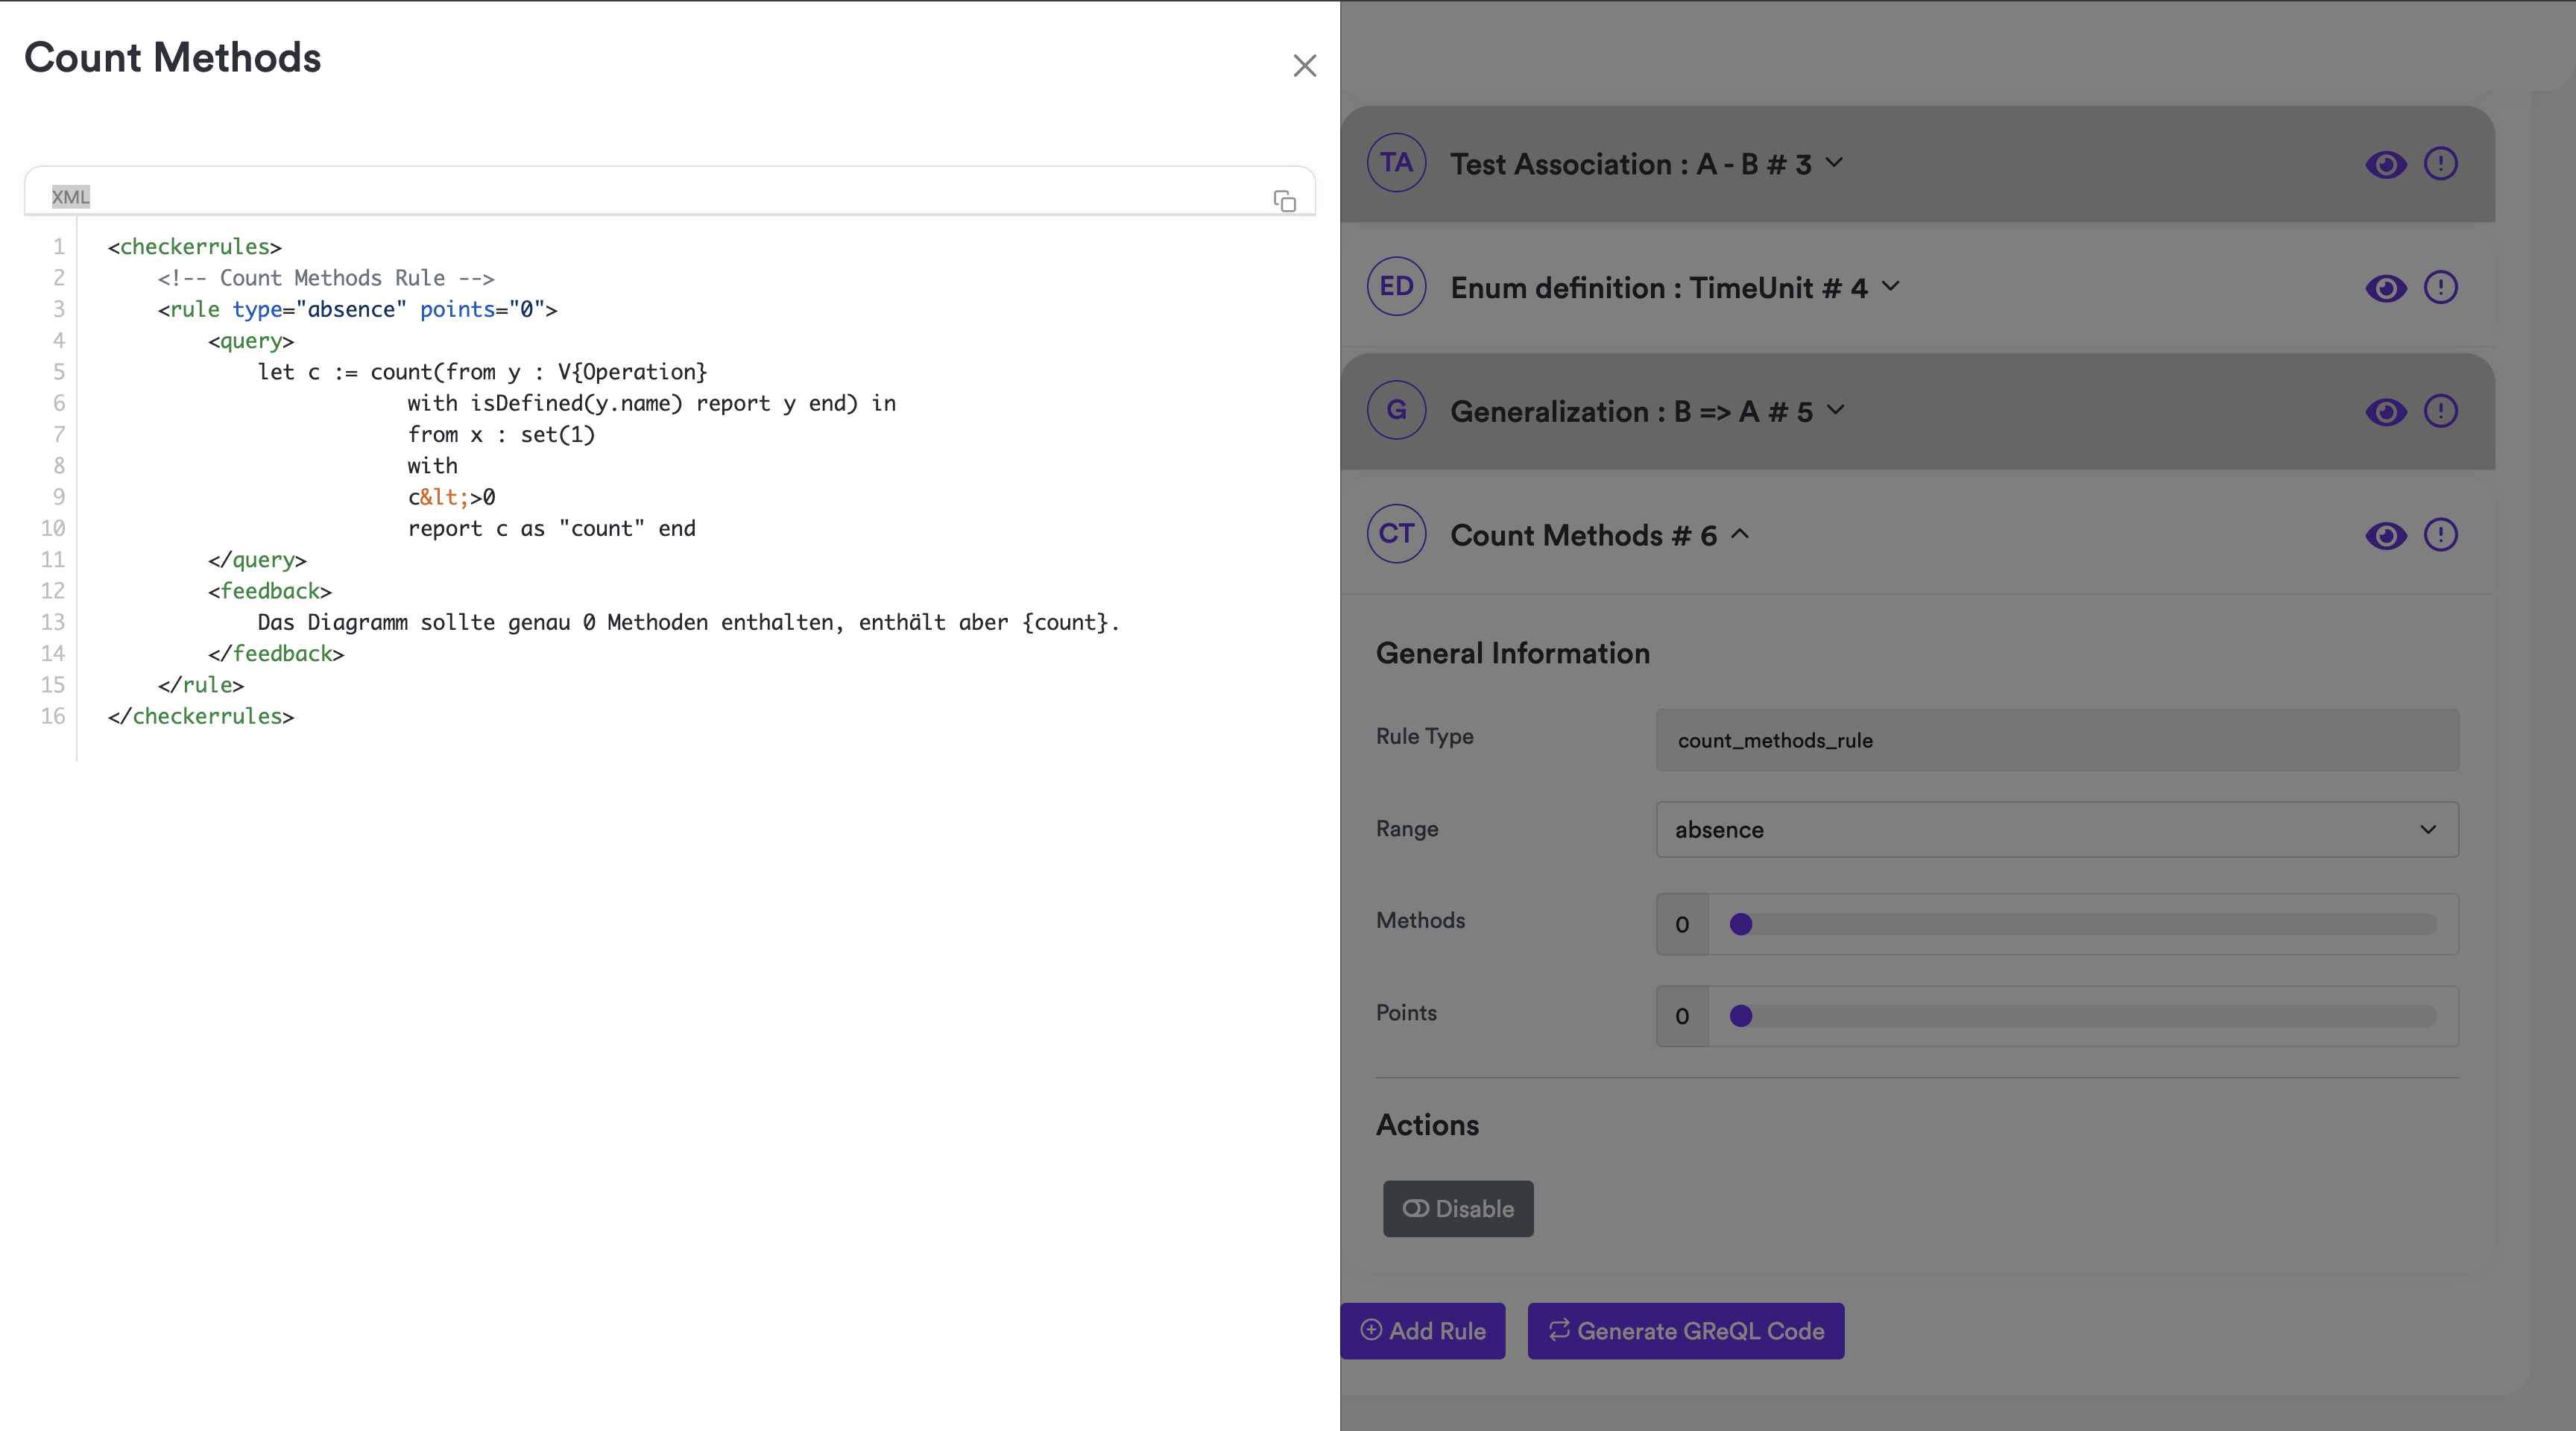
\includegraphics[width=16cm]{images/features-2n3}
    \caption{Feature 2 und 3}
    \medskip
    \small
    Auf der linken Seite des Bildes ist der GReQL-Code für die Regel ``Count Methods'' zu sehen. Um dieses Canvas
    anzuzeigen, kann man auf die Schaltfläche in Form eines Auges neben dem Titel der Regel klicken. Auf der linken
    Seite sind mehrere Regeln in Grau markiert, was bedeutet, dass sie deaktiviert sind. Diese werden daher bei der
    vollständigen Generierung des GReQL-Codes ignoriert.
    \label{fig:feat2n3}
\end{figure}

\subsection{Feature 4: Kombinierte Regeln}

Die erste Version des GReQL Converters war zweifellos sehr nützlich, da er die Erstellung einer großen Menge von Regeln
allein aus einem PlantText-Code ermöglichte. Allerdings blieb seine Nützlichkeit auf die Generierung einfacher und
größtenteils generischer Regeln beschränkt. Diese Einschränkung wurde vom Dr. Michael Striewe während seines Interviews
aufgezeigt, als er den Wunsch äußerte, komplexere Regeln aus annotiertem PlantText-Code zu generieren. Ein praktisches
Beispiel hierfür wäre zum Beispiel eine Klasse ``Bibliothek'', die ein oder mehrere Objekte der Klasse ``Buch'' enthält.
Diese einfache Darstellung kann auf verschiedene Arten modelliert werden, sei es durch das Hinzufügen von ``Buch'' als
Attribut zur Klasse ``Bibliothek``, durch Aggregation, Komposition oder einfache Beziehung. Die Einschränkung der ersten
Version des GReQL Converters bestand darin, dass er keine Möglichkeit bot, Regeln zu kombinieren, um verschiedene, aber
alle korrekte Antworten zu ermöglichen.

Um dieses Problem zu lösen, wurde die Entwicklung der Funktion zur Kombination von Regeln vorangetrieben. Diese Funktion
zielt darauf ab, eine gewisse Flexibilität zu bieten und Lehrkräften die Definition von deutlich komplexeren Regeln zu
ermöglichen. Damit können Variationen der Antworten definiert werden, die alle korrekt sein können. Um die
Funktionsweise dieser Funktionalität zu veranschaulichen, ist es sinnvoll, dies anhand eines Beispiels zu erläutern.
Angenommen, ein Lehrer möchte überprüfen, ob ein Schüler die richtige Beziehung zwischen der Klasse ``Bibliothek'' und
der Klasse ``Buch'' korrekt verwendet hat (siehe Abbildung~\ref{fig:combined}). Es gibt jedoch mehrere Möglichkeiten, wie diese
Beziehung konzipiert werden kann, wie zuvor erwähnt. Um GReQL-Code für diesen speziellen Fall zu generieren, wurde das
Annotationsystem erweitert. Durch das Stichwort ``combineID'' können Kombinationen mehrerer Regeln mit derselben
Kennung erstellt werden. Dies ermöglicht schließlich die Generierung von GReQL-Code (siehe Code~\ref{lst:combined}), der eine der
drei Bedingungen überprüft. Wenn eine dieser Bedingungen erfüllt ist, erhält der Schüler die Punkte. Details zu
diesem Annotationsystem finden sich in der Dokumentation des GReQL Converters.

\begin{figure}[h]
    \centering
    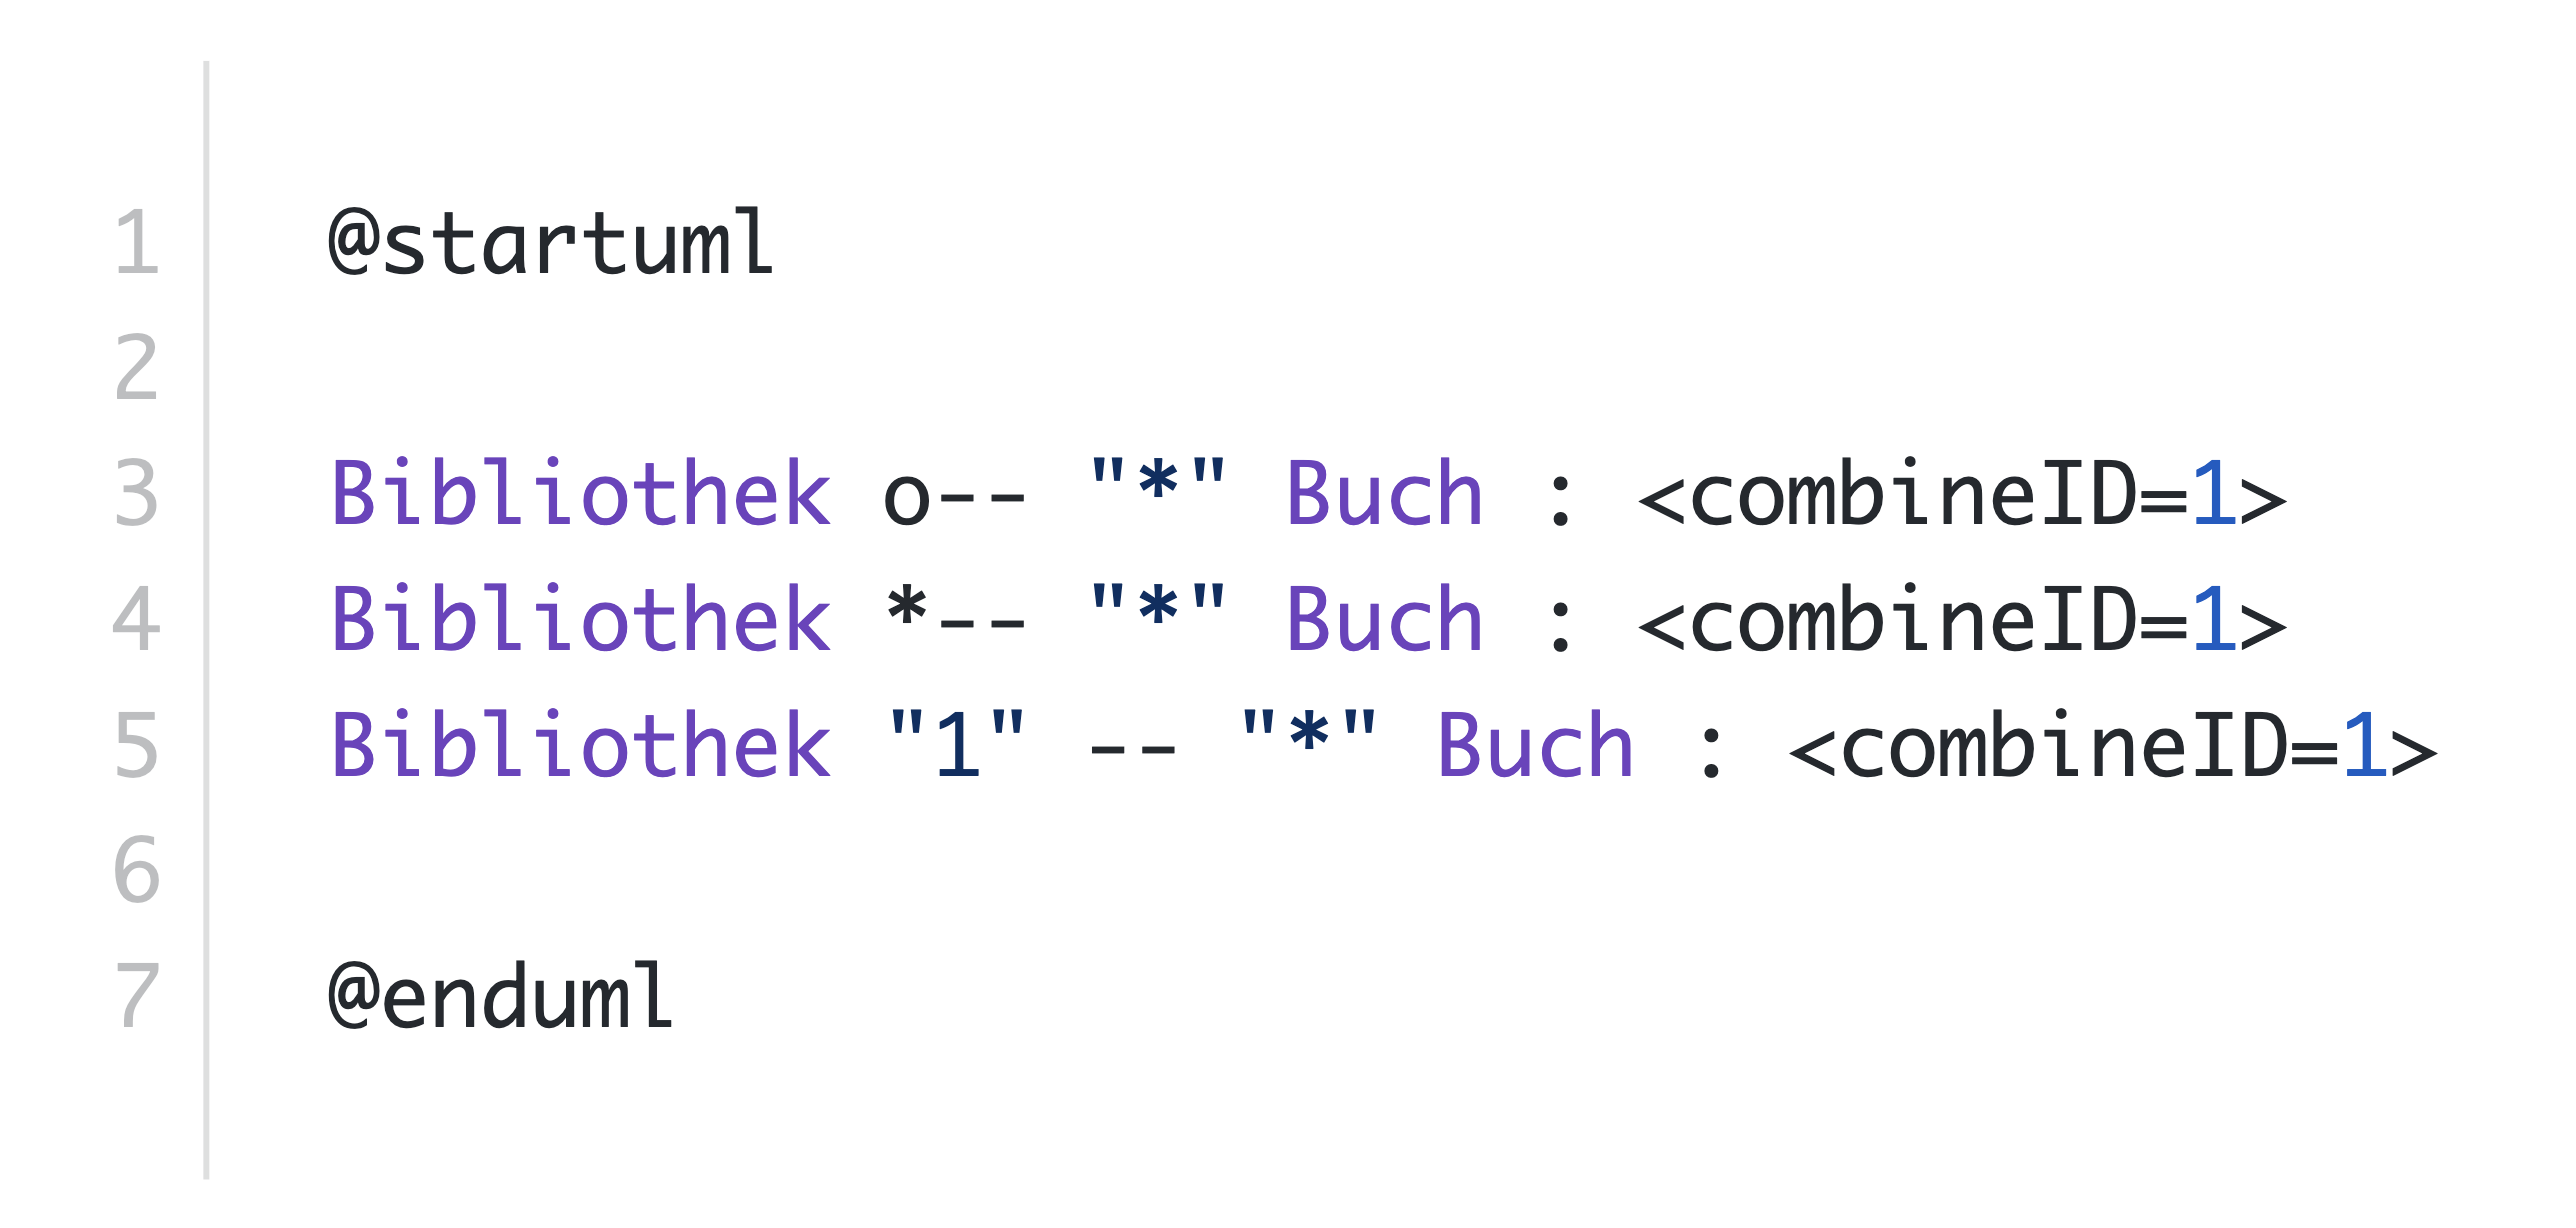
\includegraphics[width=16cm]{images/combined}
    \caption{Kombinierte Regeln}
    \label{fig:combined}
\end{figure}


\begin{lstlisting}[!h, caption={Ausschnitt aus dem GReQL-Code, der nach der Konvertierung erhalten wurde}, label={lst:combined}, language=xml]
<checkerrules>
    <!-- Combined  Rule -->

    <rule type="presence" points="0">

        <!-- Aggregation SubRule -->
        <query>
            from x, y : V{Class}, p: V{Property},
            a,b: V{LiteralString}
                with
                isDefined(x.name) and
                stringLevenshteinDistance(x.name,
                "Bibliothek")&lt;3 and
                isDefined(y.name) and
                stringLevenshteinDistance(y.name,
                "Buch")&lt;3 and
                isDefined(p.aggregation) and
                p.aggregation="shared" and
                x --> V{Property} -->
                V{Association} --> p &lt;-- y and
                isDefined(a.value) and
                a.value="*"  and
                isDefined(b.value) and
                b.value="*"  and
                x --> V{Property} --> a and
                x --> V{Property} --> b
                report 1 end
        </query>

        <!-- Composition SubRule -->
        <query>
            from x, y : V{Class}, p: V{Property},
            a,b: V{LiteralString}
                with
                isDefined(x.name) and
                stringLevenshteinDistance(x.name,
                "Bibliothek")&lt;3 and
                isDefined(y.name) and
                stringLevenshteinDistance(y.name,
                "Buch")&lt;3 and
                isDefined(p.aggregation) and
                p.aggregation="composite" and
                x --> V{Property} -->
                V{Association} --> p &lt;-- y and
                isDefined(a.value) and
                a.value="*"  and
                isDefined(b.value) and
                b.value="*"  and
                x --> V{Property} --> a and
                x --> V{Property} --> b
                report 1 end
        </query>

        <!-- Simple Association SubRule -->
        <query>
            from x,y : V{Class}, ass : V{Association},
            a,b,c,d  : V{LiteralString}
                with
                isDefined(x.name) and
                stringLevenshteinDistance(x.name,
                "Bibliothek")&lt;3 and
                isDefined(y.name) and
                stringLevenshteinDistance(y.name,
                "Buch")&lt;3 and
                isDefined(a.value) and
                a.value="*"  and
                isDefined(b.value) and
                b.value="*"  and
                x --> V{Property} --> a and
                x --> V{Property} --> b and
                isDefined(c.value) and
                c.value="1"  and
                isDefined(d.value) and
                d.value="1"  and
                y --> V{Property} --> c and
                y --> V{Property} --> d and
                x --> V{Property} --> ass
                &lt;-- V{Property} &lt;-- y
                report 1 end
        </query>
        <feedback>
            ... i need a feedback please 😊.
        </feedback>
    </rule>
</checkerrules>
\end{lstlisting}

\section{Zusammenfassung der Evaluation}

Abschließend bietet die Analyse und Bewertung des GReQL Converters einen detaillierten Einblick in die Wirksamkeit und
Potenziale dieses Tools. Die erörterten Verbesserungsvorschläge sowie die ermittelten Stärken und Schwächen legen den
Grundstein für zukünftige Entwicklungen und zeigen auf, wie dieses Instrument im Bildungsumfeld und darüber hinaus noch
effektiver genutzt werden könnte. Die Bewertung des Tools, getragen von den Erwartungen, dem Nutzen und den
Erkenntnissen aus den Anwendererfahrungen, bildet eine solide Grundlage für weiterführende Studien und Implementierungen
zur Steigerung seiner Funktionalitäten und Anwenderfreundlichkeit. Diese umfassende Bewertung legt den Fokus auf die
kontinuierliche Weiterentwicklung und Optimierung des GReQL Converters, um seinen Wert und seine Wirksamkeit für
zukünftige Anwendungen zu maximieren.
